\chapter{Introducción Específica} % Main chapter title

\label{Chapter2}

%----------------------------------------------------------------------------------------
%	SECTION 1
%----------------------------------------------------------------------------------------
En este capítulo se realiza una descripción del planeamiento y estructura del trabajo, sus requerimientos y características principales.

\section{Estructura del trabajo}
\label{sec:cap2parte1}
Inicialmente se realizó un plan de trabajo donde se plantea cómo se afronta el problema y el modo en que se lo resolverá. El proyecto consta de dos partes principales: hardware y software.

Para el hardware se planteó un diagrama de bloques que sirvió de guía al realizar el esquemático, que puede verse en la figura \ref{fig:bloquess1}. El diagrama plantea dos sectores uno de procesamiento y otro de medición que se encontraran aislados.

\begin{figure}[h]
	\centering
	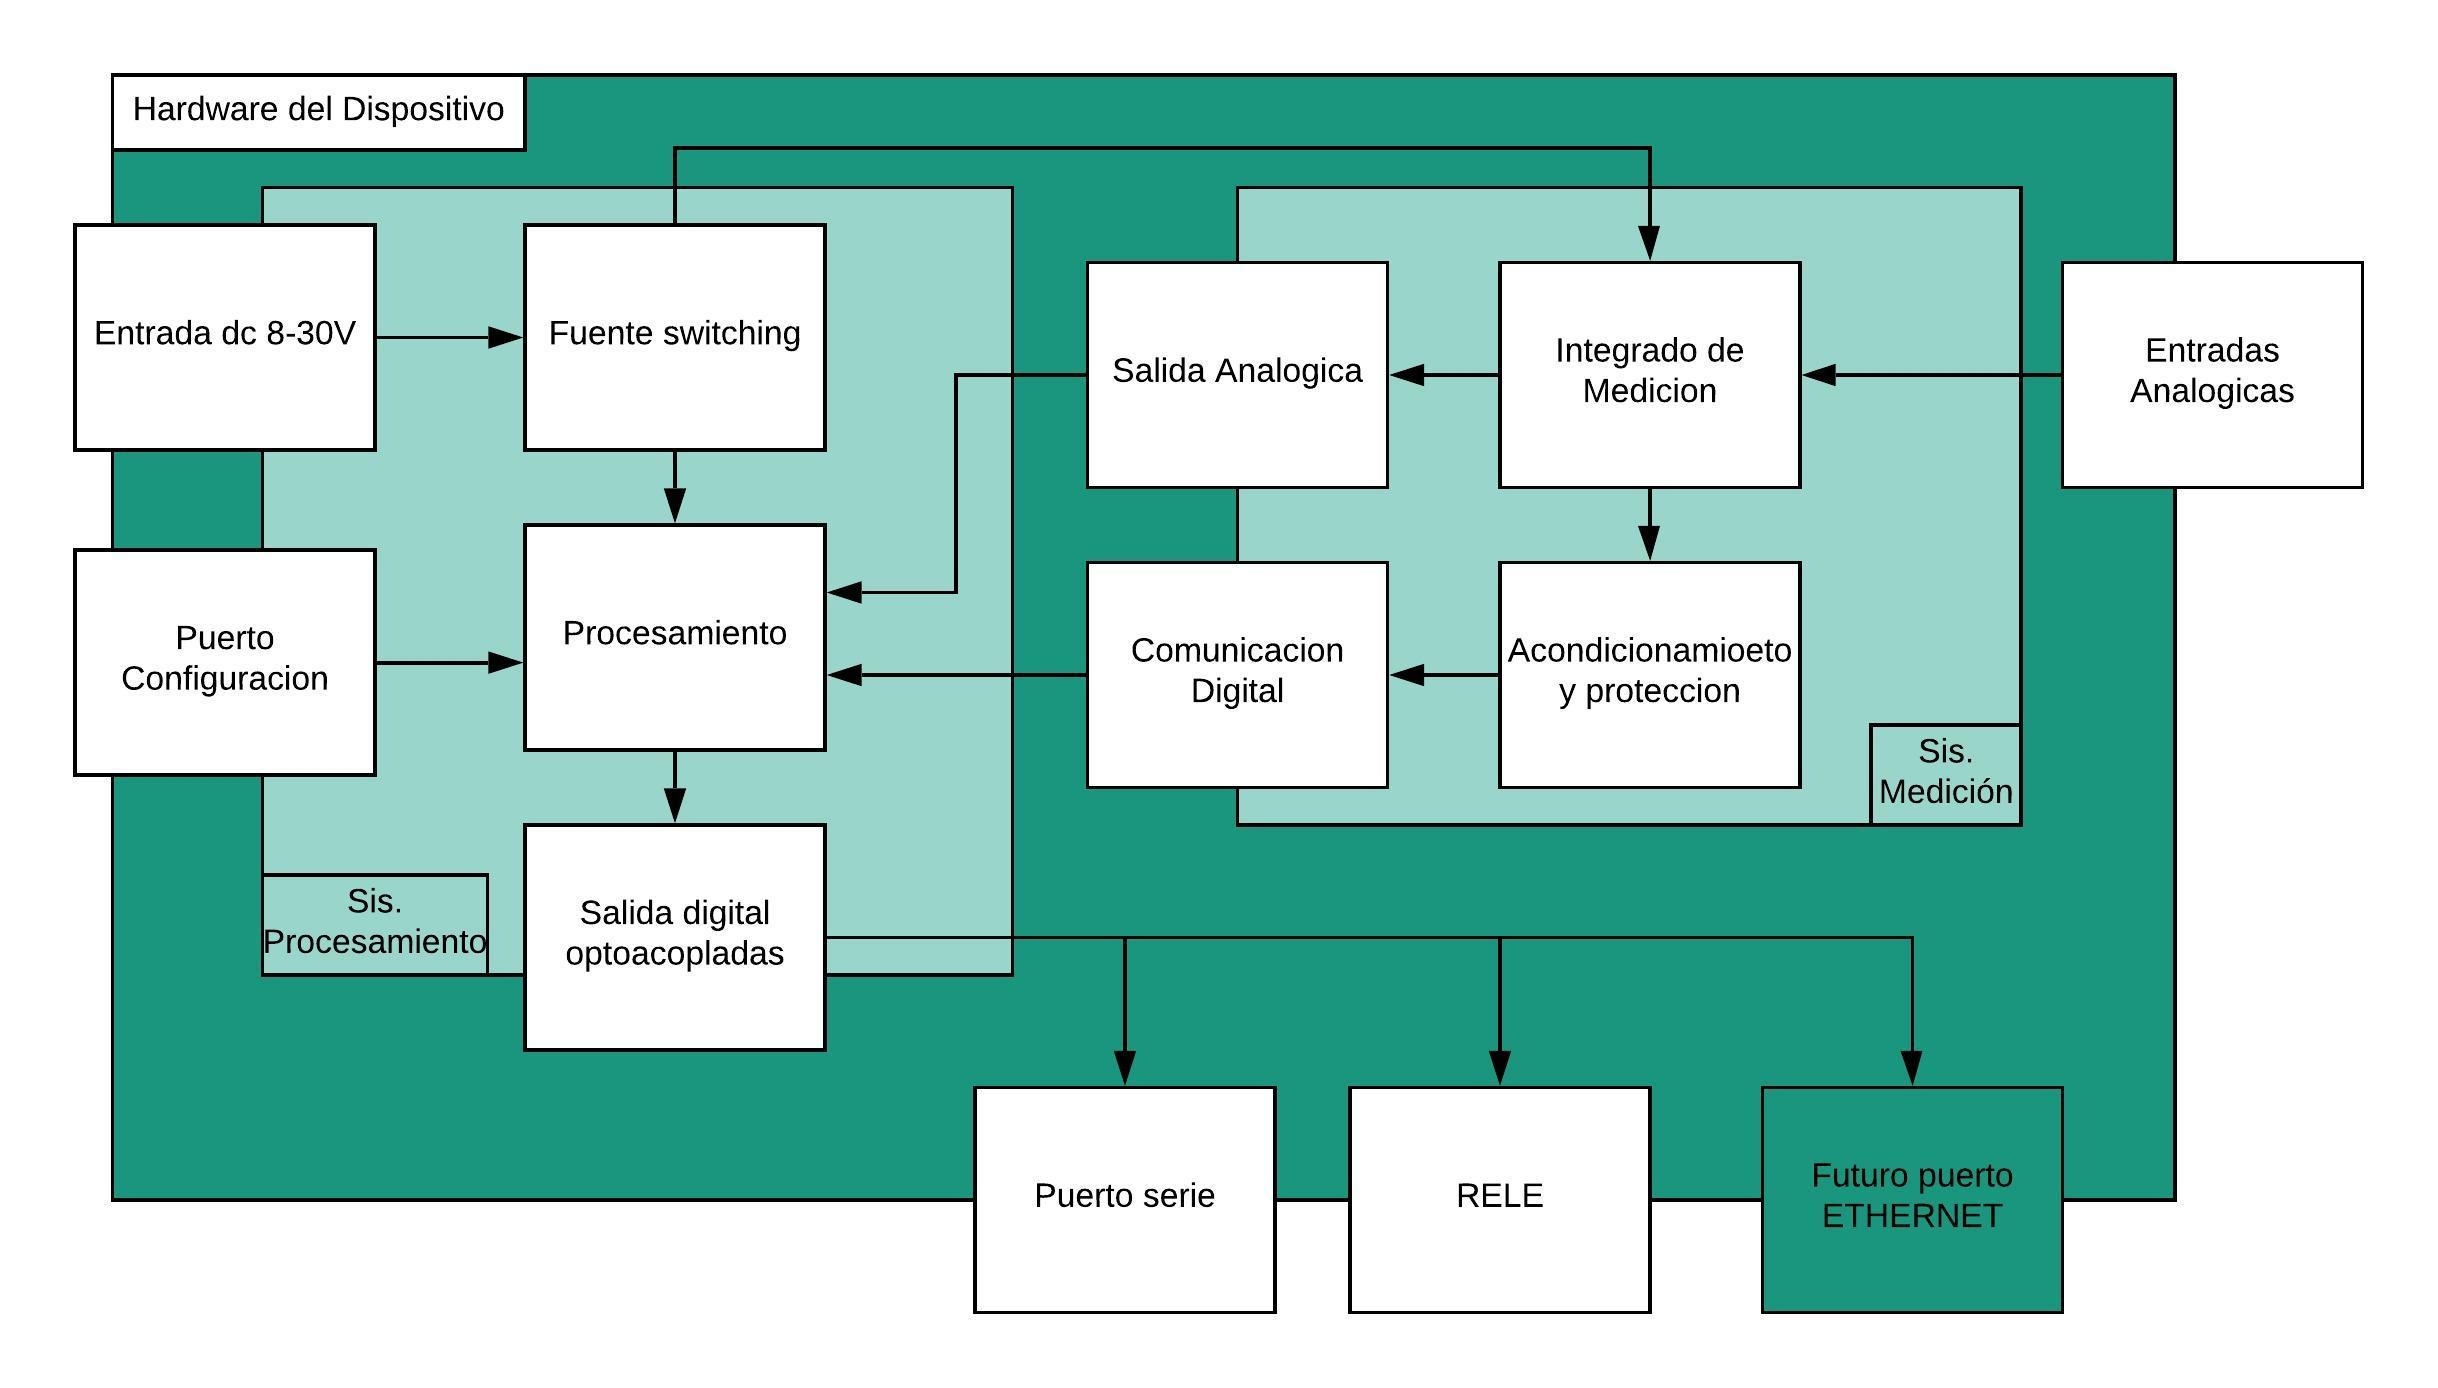
\includegraphics[width=120mm,keepaspectratio]{Figures/concepto.jpeg}
	\caption{Diagrama planteado para la elaboración de hardware.}
	\label{fig:bloquess1}
\end{figure}

El diagrama presupone que se usará una entrada de alimentación de corriente continua de 8 a 30 V conectado a una una fuente \textit{switching}, alimentando tanto al procesamiento como a la medición.

Del sistema de procesamiento se tiene que el hardware contara con un puerto de configuración y varias salidas optoacopladas, se plantea que estas salidas sean un relé ,un puerto serie y un puerto ethernet.

Del sistema de medición se observa comunicar al procesamiento por una comunicación digital aislada y también por una salida analógica. También se indica que la medición tendrá varias entradas analógicas, pero estas no fueron especificadas.

En cuanto el software se estableció que sea el necesario para lograr el testeo de las partes del hardware y la verificación de los requerimientos, por lo que el software debía manejar correctamente todos los integrados que fueran a estar embebidos en el circuito del dispositivo y manejar todos los protocolos definidos en los requisitos.

El enfoque inicial del trabajo fue el armado de la electrónica del prototipo, y el software se constituyó como la segunda parte que debía demostrar el correcto funcionamiento del hardware.

\section{Requerimientos del trabajo}
\label{sec:cap2parte2}
Los requerimientos fueron elaborados a partir de un documento enviado por el equipo de desarrollo de la empresa. Pueden verse en la siguiente lista:

\begin{itemize}
\item Grupo de requerimientos referidos a medición de potencia del equipo:
\begin{enumerate}
\item El dispositivo debe ser capaz de realizar la medición de tensión alterna de una línea monofásica de baja tensión de Argentina, entrada de medición para 220 V o 380 V con una tolerancia de +/-15\%.
\item El dispositivo debe ser capaz de realizar la medición de corriente alterna de una línea monofásica de baja tensión de Argentina, hasta 5 A.
\item El dispositivo debe ser capaz de realizar la medición de potencia eléctrica activa de una línea monofásica de baja tensión de Argentina, hasta 4000 W.
\item El sistema de medición que se utiliza para las mediciones debe ser aislado de la salida de comunicaciones del puerto serie.
\end{enumerate}

\item Grupo de requerimientos referidos a Interfaces de comunicación:
\begin{enumerate}
\setcounter{enumi}{4}
\item El dispositivo debe realizar las comunicaciones a través de protocolos RS485 y RS232.
\item El dispositivo debe tener en su diseño espacio para una posible modificación a futuro en la que se incluya una interfaz ethernet a través de una entrada para rj45.
\end{enumerate}

\item Grupo de requerimientos referidos a diseño del circuito eléctrico:
\begin{enumerate}
\setcounter{enumi}{6}
\item El dispositivo debe alimentarse con tensión continua que debe ser inferior a 30 V y superior a 12 V.
\item El dispositivo debe poseer como microcontrolador principal MSP430F2418.
\item El dispositivo debe implementar protecciones contra sobretensión en salida y entradas.
\item El dspositivo debe tener un relé para realizar un corte por corriente.
\end{enumerate}

\item Grupo de requerimientos referidos a diseño  de impresión del circuito:
\begin{enumerate}
\setcounter{enumi}{10}
\item El tipo de soldado debe ser por refusión en la cara superior del circuito impreso.

\item El tipo de soldado debe ser por ola en la cara inferior del circuito impreso.
\end{enumerate}
\end{itemize}




%\subsection{Uso de mayúscula inicial para los título de secciones}
